\subsubsection{Gradientenindexprofil (GI-POF)}

Das Gradientenindexprofil bittet mit bis zu 40 Gigabit/s auf 100m deutlich
höhere Bitraten als das Stufenindexprofil. Beim Gradientenindex nimmt der
Brechungsindex vom Mantel bis zur Mitte des Kern kontinuierlich zu (siehe
\autoref{fig:pofgi} Spalte Brechungsindex). \autoref{fig:pofgi} zeigt ebenfalls
in der Spalte Längsschnitt den daraus resultierenden Lichtstrahlenverlauf.
Dieser verläuft, im Gegensatz zu der geraden Lichtausbreitung beim Stufenindex,
sinusförmig. Der Kerndurchmesser der GI-POF ist mit ca. 100 µm um das 10fache
geringer als der einer SI-POF. Dadurch werden geringere Laufzeitunterschiede
ermöglicht und die Frequenz der Lichtimpulse kann erhöht werden. Außerdem wird
bei der GI-POF eine Dämpfung von unter 20 dB/km erreicht. Dies ist eine
ehrheblicher Verbesserung gegenüber der Dämpfung von SI-POF mit ca. 100 dB/km
(siehe \autoref{fig:pofgidaempfung}). Aus den beiden Gründen ist die Bandbreite
einer Faser mit Gradientenindex significant höher als die einer einer Faser mit
Stufenindex. Als Kernmaterial kann hier der Kunststoff
CYTOP\textsuperscript{\texttrademark} der Asahi Glass Co., Ltd. oder
Polymethylmethacrylat verwendet werden \cite{pofacgif}. Aufgrund der hohen
Bitraten und der Biegsamkeit werden GI-POF in \shorthandoff{"}"Local Area
Networks"\shorthandon{"} (LAN) und in Supercomputern eingesetzt \cite{poflee}.

\begin{figure}[h]
    \begin{center}
        \begin{minipage}[t]{0.4\textwidth}
            \begin{center}
                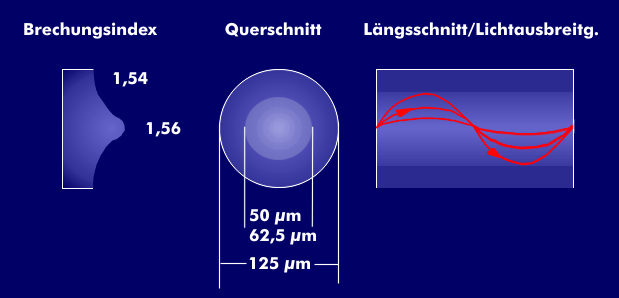
\includegraphics[width=0.9\textwidth]{Bilder/Optische_Wellenleiter_Die_Polymer_Optische_Faser/Brechzahlprofile/pofgi.png}
                \caption[Aufbau des Gradientenindexprofils \newline \url{http://www.itwissen.info/bilder/aufbau-und-brechungsprofil-der-gradientenfaser.png} (zuletzt aufgerufen am 19.09.2015)]{Aufbau des Gradientenindexprofils}
                \label{fig:pofgi}
            \end{center}
        \end{minipage}
        \hspace{0.025\textwidth}
        \begin{minipage}[t]{0.4\textwidth}
            \begin{center}
                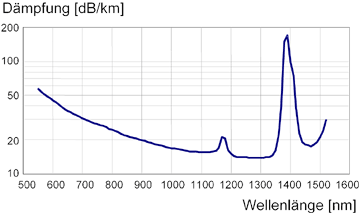
\includegraphics[height=0.1\textheight]{Bilder/Optische_Wellenleiter_Die_Polymer_Optische_Faser/Brechzahlprofile/pofgidaempfung.png}
                \caption[Dämpfung bei einer GI-POF \newline \url{http://www.pofac.fh-nuernberg.de/pofac/de/was_sind_pof/images/gradientenindex_daempfung.png} (zuletzt aufgerufen am 19.09.2015)]{Vergleich der Dämpfungswerte von GI-POF und SI-POF}
                \label{fig:pofgidaempfung}
            \end{center}
        \end{minipage}
    \end{center}
\end{figure}
